% Appendix: results at every cutoff.
\section{Results at Every Cutoff}
\label{app:full-results}

\ifdefined\nwvtwo% T2: main comparison (two-column table*). Means over cutoffs; every cell is in Appendix E.
% The decontaminated block is tables/t2b-decon.tex, read only under \nwdecontrue.
\begin{table*}[t]
\centering\small
\setlength{\tabcolsep}{2.4pt}
\begin{tabular}{@{}llccccrr@{}}
\toprule
 &  & \multicolumn{1}{c}{\nwhead{Recall}} & \multicolumn{1}{c}{\nwhead{Precision}} & \multicolumn{1}{c}{\nwhead{Citation}} & \nwhead{Later facts} & \nwhead{Distinct} & \nwhead{Tokens} \\
\multicolumn{2}{@{}l}{\nwhead{System (cutoff enforced by)}} & \multicolumn{1}{c}{\nwhead{$\uparrow$}} & \multicolumn{1}{c}{\nwhead{$\uparrow$}} & \multicolumn{1}{c}{\nwhead{sufficiency $\uparrow$}} & \nwhead{disclosed $\downarrow$} & \nwhead{assertions} & \nwhead{in / out (M)} \\
\midrule
B1 & Long context (input) & \cellcolor{nwhighcyan}\best{\res{M1-anne-avg-B1}}\sdev{\res{STAT-M1-B1-sd}} & \res{M3-anne-avg-B1}\sdev{\res{STAT-M3-B1-sd}} & \res{M8-anne-avg-B1}\sdev{\res{STAT-M8-B1-sd}} & \res{M4-anne-total-B1} & \res{ND-anne-avg-B1} & \res{TOK-anne-B1} \\
B2 & Prefix retrieval (input) & \res{M1-anne-avg-B2}\sdev{\res{STAT-M1-B2-sd}} & \res{M3-anne-avg-B2}\sdev{\res{STAT-M3-B2-sd}} & \res{M8-anne-avg-B2}\sdev{\res{STAT-M8-B2-sd}} & \res{M4-anne-total-B2} & \res{ND-anne-avg-B2} & \cellcolor{nwhighlavender}\best{\res{TOK-anne-B2}} \\
B3 & LightRAG (input) & \res{M1-anne-avg-B3}\sdev{\res{STAT-M1-B3-sd}} & \res{M3-anne-avg-B3}\sdev{\res{STAT-M3-B3-sd}} & \res{M8-anne-avg-B3}\sdev{\res{STAT-M8-B3-sd}} & \res{M4-anne-total-B3} & \res{ND-anne-avg-B3} & \res{TOK-anne-B3} \\
B4 & Graph baseline & \res{M1-anne-avg-B4}\sdev{\res{STAT-M1-B4-sd}} & \cellcolor{nwhighcyan}\best{\res{M3-anne-avg-B4}}\sdev{\res{STAT-M3-B4-sd}} & \cellcolor{nwhighcyan}\best{\res{M8-anne-avg-B4}}\sdev{\res{STAT-M8-B4-sd}} & \res{M4-anne-total-B4} & \res{ND-anne-avg-B4} & +\res{TOK-anne-B4} \\
B5 & \sys (data) & \res{M1-anne-avg-B5}\sdev{\res{STAT-M1-B5-sd}} & \res{M3-anne-avg-B5}\sdev{\res{STAT-M3-B5-sd}} & \res{M8-anne-avg-B5}\sdev{\res{STAT-M8-B5-sd}} & \cellcolor{nwhighpink}\best{\res{M4-anne-total-B5}} & \cellcolor{nwhighlavender}\best{\res{ND-anne-avg-B5}} & \res{TOK-anne-B5} \\
\midrule
X1 & Closed book (none) & \res{M1-anne-avg-X1}\sdev{\res{STAT-M1-X1-sd}} & \res{M3-anne-avg-X1}\sdev{\res{STAT-M3-X1-sd}} & -- & \cellcolor{nwhighpink}\best{\res{M4-anne-total-X1}} & \res{ND-anne-avg-X1} & \res{TOK-anne-X1} \\
X2 & Full text (instruction) & \res{M1-anne-avg-X2}\sdev{\res{STAT-M1-X2-sd}} & \res{M3-anne-avg-X2}\sdev{\res{STAT-M3-X2-sd}} & \res{M8-anne-avg-X2}\sdev{\res{STAT-M8-X2-sd}} & \cellcolor{nwhighpink}\best{\res{M4-anne-total-X2}} & \res{ND-anne-avg-X2} & \res{TOK-anne-X2} \\
\bottomrule
\end{tabular}
\caption{Main comparison on Anne: rates are mean $\pm$ sample standard deviation across
$t=1..5$. Recall uses eligible gold facts; precision and citation sufficiency use 40 sampled
atoms per cutoff, judged in page context. Disclosure counts stated or implied later facts
across $t=1..4$. Distinct assertions are means per cutoff; tokens (millions, input / output)
cover the reported build. X1 and X2
are diagnostics; X1 cites nothing. Bold identifies rate and assertion-count maxima and
minimum measured cost among B1--B5, plus non-zero disclosures. Cyan highlights performance
maxima, pink disclosures, and lavender inventory and minimum cost. B4 reuses B5's graph;
its cell is the page generation added to B5's build. Distributions are in Table~\ref{tab:stats}.}
\label{tab:main}
\end{table*}
\fi % v2: Table tab:main lives here
% Appendix E: every cutoff x system on the evaluated work (B4 is in Appendix G, tab:b4).
\begin{table*}[t]
\centering\small
\setlength{\tabcolsep}{4pt}
\begin{tabular}{@{}clccccr@{}}
\toprule
\nwhead{$t$} & \nwhead{System} & \nwhead{Recall (M1)} & \nwhead{Precision (M3)} & \nwhead{Citation sufficiency (M8)} & \nwhead{Disclosed (M4)} & \nwhead{Assertions} \\
\midrule
1 & B1 & \res{M1-anne-t1-B1} & \res{M3-anne-t1-B1} & \res{M8-anne-t1-B1} & \res{M4-anne-t1-B1} & \res{N-anne-t1-B1} \\
 & B2 & \cellcolor{nwhighcyan}\best{\res{M1-anne-t1-B2}} & \res{M3-anne-t1-B2} & \cellcolor{nwhighcyan}\best{\res{M8-anne-t1-B2}} & \res{M4-anne-t1-B2} & \res{N-anne-t1-B2} \\
 & B3 & \res{M1-anne-t1-B3} & \cellcolor{nwhighcyan}\best{\res{M3-anne-t1-B3}} & \res{M8-anne-t1-B3} & \res{M4-anne-t1-B3} & \res{N-anne-t1-B3} \\
 & \sys & \res{M1-anne-t1-B5} & \res{M3-anne-t1-B5} & \res{M8-anne-t1-B5} & \res{M4-anne-t1-B5} & \cellcolor{nwhighlavender}\best{\res{N-anne-t1-B5}} \\
 & X1 & \res{M1-anne-t1-X1} & \res{M3-anne-t1-X1} & -- & \cellcolor{nwhighpink}\best{\res{M4-anne-t1-X1}} & \res{N-anne-t1-X1} \\
 & X2 & \res{M1-anne-t1-X2} & \res{M3-anne-t1-X2} & \res{M8-anne-t1-X2} & \res{M4-anne-t1-X2} & \res{N-anne-t1-X2} \\
\midrule
2 & B1 & \cellcolor{nwhighcyan}\best{\res{M1-anne-t2-B1}} & \res{M3-anne-t2-B1} & \res{M8-anne-t2-B1} & \res{M4-anne-t2-B1} & \res{N-anne-t2-B1} \\
 & B2 & \res{M1-anne-t2-B2} & \cellcolor{nwhighcyan}\best{\res{M3-anne-t2-B2}} & \res{M8-anne-t2-B2} & \res{M4-anne-t2-B2} & \res{N-anne-t2-B2} \\
 & B3 & \res{M1-anne-t2-B3} & \res{M3-anne-t2-B3} & \cellcolor{nwhighcyan}\best{\res{M8-anne-t2-B3}} & \res{M4-anne-t2-B3} & \res{N-anne-t2-B3} \\
 & \sys & \res{M1-anne-t2-B5} & \res{M3-anne-t2-B5} & \res{M8-anne-t2-B5} & \res{M4-anne-t2-B5} & \cellcolor{nwhighlavender}\best{\res{N-anne-t2-B5}} \\
 & X1 & \res{M1-anne-t2-X1} & \res{M3-anne-t2-X1} & -- & \cellcolor{nwhighpink}\best{\res{M4-anne-t2-X1}} & \res{N-anne-t2-X1} \\
 & X2 & \res{M1-anne-t2-X2} & \res{M3-anne-t2-X2} & \res{M8-anne-t2-X2} & \cellcolor{nwhighpink}\best{\res{M4-anne-t2-X2}} & \res{N-anne-t2-X2} \\
\midrule
3 & B1 & \cellcolor{nwhighcyan}\best{\res{M1-anne-t3-B1}} & \cellcolor{nwhighcyan}\best{\res{M3-anne-t3-B1}} & \res{M8-anne-t3-B1} & \res{M4-anne-t3-B1} & \res{N-anne-t3-B1} \\
 & B2 & \res{M1-anne-t3-B2} & \cellcolor{nwhighcyan}\best{\res{M3-anne-t3-B2}} & \cellcolor{nwhighcyan}\best{\res{M8-anne-t3-B2}} & \res{M4-anne-t3-B2} & \res{N-anne-t3-B2} \\
 & B3 & \res{M1-anne-t3-B3} & \cellcolor{nwhighcyan}\best{\res{M3-anne-t3-B3}} & \res{M8-anne-t3-B3} & \res{M4-anne-t3-B3} & \res{N-anne-t3-B3} \\
 & \sys & \res{M1-anne-t3-B5} & \res{M3-anne-t3-B5} & \res{M8-anne-t3-B5} & \cellcolor{nwhighpink}\best{\res{M4-anne-t3-B5}} & \cellcolor{nwhighlavender}\best{\res{N-anne-t3-B5}} \\
 & X1 & \res{M1-anne-t3-X1} & \res{M3-anne-t3-X1} & -- & \res{M4-anne-t3-X1} & \res{N-anne-t3-X1} \\
 & X2 & \res{M1-anne-t3-X2} & \res{M3-anne-t3-X2} & \res{M8-anne-t3-X2} & \res{M4-anne-t3-X2} & \res{N-anne-t3-X2} \\
\midrule
4 & B1 & \res{M1-anne-t4-B1} & \res{M3-anne-t4-B1} & \res{M8-anne-t4-B1} & \res{M4-anne-t4-B1} & \res{N-anne-t4-B1} \\
 & B2 & \cellcolor{nwhighcyan}\best{\res{M1-anne-t4-B2}} & \res{M3-anne-t4-B2} & \res{M8-anne-t4-B2} & \res{M4-anne-t4-B2} & \res{N-anne-t4-B2} \\
 & B3 & \res{M1-anne-t4-B3} & \cellcolor{nwhighcyan}\best{\res{M3-anne-t4-B3}} & \cellcolor{nwhighcyan}\best{\res{M8-anne-t4-B3}} & \res{M4-anne-t4-B3} & \res{N-anne-t4-B3} \\
 & \sys & \res{M1-anne-t4-B5} & \res{M3-anne-t4-B5} & \res{M8-anne-t4-B5} & \res{M4-anne-t4-B5} & \cellcolor{nwhighlavender}\best{\res{N-anne-t4-B5}} \\
 & X1 & \res{M1-anne-t4-X1} & \res{M3-anne-t4-X1} & -- & \cellcolor{nwhighpink}\best{\res{M4-anne-t4-X1}} & \res{N-anne-t4-X1} \\
 & X2 & \res{M1-anne-t4-X2} & \res{M3-anne-t4-X2} & \res{M8-anne-t4-X2} & \cellcolor{nwhighpink}\best{\res{M4-anne-t4-X2}} & \res{N-anne-t4-X2} \\
\midrule
5 & B1 & \res{M1-anne-t5-B1} & \res{M3-anne-t5-B1} & \res{M8-anne-t5-B1} & -- & \res{N-anne-t5-B1} \\
 & B2 & \cellcolor{nwhighcyan}\best{\res{M1-anne-t5-B2}} & \cellcolor{nwhighcyan}\best{\res{M3-anne-t5-B2}} & \res{M8-anne-t5-B2} & -- & \res{N-anne-t5-B2} \\
 & B3 & \res{M1-anne-t5-B3} & \res{M3-anne-t5-B3} & \cellcolor{nwhighcyan}\best{\res{M8-anne-t5-B3}} & -- & \res{N-anne-t5-B3} \\
 & \sys & \res{M1-anne-t5-B5} & \res{M3-anne-t5-B5} & \res{M8-anne-t5-B5} & -- & \cellcolor{nwhighlavender}\best{\res{N-anne-t5-B5}} \\
 & X1 & \res{M1-anne-t5-X1} & \res{M3-anne-t5-X1} & -- & -- & \res{N-anne-t5-X1} \\
 & X2 & \res{M1-anne-t5-X2} & \res{M3-anne-t5-X2} & \res{M8-anne-t5-X2} & -- & \res{N-anne-t5-X2} \\
\bottomrule
\end{tabular}
\caption{Results at every cutoff. Rates are followed by their counts. Disclosure is the number of
assessed later facts stated or implied over $|\Ft|$ and is undefined at $t=5$; citation
sufficiency has no value for X1, which cites nothing; assertions is the size of the cutoff's assertion
inventory, counting a statement once for every page that prints it. A precision denominator
below 40 reflects excluded frame errors. B4 is reported in Table~\ref{tab:b4}.
Bold: highest rates and assertion count at each cutoff among B1, B2, B3 and B5, and each
non-zero disclosure count. Cyan, pink, and lavender highlight performance maxima,
disclosures, and assertion counts, respectively.}
\label{tab:full-results}
\end{table*}

% Generated by scripts/papers/summary_stats.py from the per-cutoff keys in results.tex. Do not edit.
\begin{table*}[t]
\centering\footnotesize
\setlength{\tabcolsep}{2pt}
% Systems across columns (transposed).
\begin{minipage}[t]{0.49\textwidth}
\centering
\textbf{Recall} ($n=5$)\par\smallskip
\begin{tabular}{@{}lrrrrrrr@{}}
\toprule
\nwhead{Statistic} & \nwhead{B1} & \nwhead{B2} & \nwhead{B3} & \nwhead{B4} & \nwhead{B5} & \nwhead{X1} & \nwhead{X2} \\
\midrule
Mean & \cellcolor{nwhighcyan}\best{\res{STAT-M1-B1-mean}} & \res{STAT-M1-B2-mean} & \res{STAT-M1-B3-mean} & \res{STAT-M1-B4-mean} & \res{STAT-M1-B5-mean} & \res{STAT-M1-X1-mean} & \res{STAT-M1-X2-mean} \\
SD & \res{STAT-M1-B1-sd} & \res{STAT-M1-B2-sd} & \res{STAT-M1-B3-sd} & \res{STAT-M1-B4-sd} & \res{STAT-M1-B5-sd} & \res{STAT-M1-X1-sd} & \res{STAT-M1-X2-sd} \\
Median & \res{STAT-M1-B1-median} & \res{STAT-M1-B2-median} & \res{STAT-M1-B3-median} & \res{STAT-M1-B4-median} & \res{STAT-M1-B5-median} & \res{STAT-M1-X1-median} & \res{STAT-M1-X2-median} \\
Min & \res{STAT-M1-B1-min} & \res{STAT-M1-B2-min} & \res{STAT-M1-B3-min} & \res{STAT-M1-B4-min} & \res{STAT-M1-B5-min} & \res{STAT-M1-X1-min} & \res{STAT-M1-X2-min} \\
Max & \res{STAT-M1-B1-max} & \res{STAT-M1-B2-max} & \res{STAT-M1-B3-max} & \res{STAT-M1-B4-max} & \res{STAT-M1-B5-max} & \res{STAT-M1-X1-max} & \res{STAT-M1-X2-max} \\
\bottomrule
\end{tabular}
\end{minipage}
\hfill
\begin{minipage}[t]{0.49\textwidth}
\centering
\textbf{Precision} ($n=5$)\par\smallskip
\begin{tabular}{@{}lrrrrrrr@{}}
\toprule
\nwhead{Statistic} & \nwhead{B1} & \nwhead{B2} & \nwhead{B3} & \nwhead{B4} & \nwhead{B5} & \nwhead{X1} & \nwhead{X2} \\
\midrule
Mean & \res{STAT-M3-B1-mean} & \res{STAT-M3-B2-mean} & \res{STAT-M3-B3-mean} & \cellcolor{nwhighcyan}\best{\res{STAT-M3-B4-mean}} & \res{STAT-M3-B5-mean} & \res{STAT-M3-X1-mean} & \res{STAT-M3-X2-mean} \\
SD & \res{STAT-M3-B1-sd} & \res{STAT-M3-B2-sd} & \res{STAT-M3-B3-sd} & \res{STAT-M3-B4-sd} & \res{STAT-M3-B5-sd} & \res{STAT-M3-X1-sd} & \res{STAT-M3-X2-sd} \\
Median & \res{STAT-M3-B1-median} & \res{STAT-M3-B2-median} & \res{STAT-M3-B3-median} & \res{STAT-M3-B4-median} & \res{STAT-M3-B5-median} & \res{STAT-M3-X1-median} & \res{STAT-M3-X2-median} \\
Min & \res{STAT-M3-B1-min} & \res{STAT-M3-B2-min} & \res{STAT-M3-B3-min} & \res{STAT-M3-B4-min} & \res{STAT-M3-B5-min} & \res{STAT-M3-X1-min} & \res{STAT-M3-X2-min} \\
Max & \res{STAT-M3-B1-max} & \res{STAT-M3-B2-max} & \res{STAT-M3-B3-max} & \res{STAT-M3-B4-max} & \res{STAT-M3-B5-max} & \res{STAT-M3-X1-max} & \res{STAT-M3-X2-max} \\
\bottomrule
\end{tabular}
\end{minipage}
\par\medskip
\begin{minipage}[t]{0.49\textwidth}
\centering
\textbf{Citation sufficiency} ($n=5$)\par\smallskip
\begin{tabular}{@{}lrrrrrrr@{}}
\toprule
\nwhead{Statistic} & \nwhead{B1} & \nwhead{B2} & \nwhead{B3} & \nwhead{B4} & \nwhead{B5} & \nwhead{X1} & \nwhead{X2} \\
\midrule
Mean & \res{STAT-M8-B1-mean} & \res{STAT-M8-B2-mean} & \res{STAT-M8-B3-mean} & \cellcolor{nwhighcyan}\best{\res{STAT-M8-B4-mean}} & \res{STAT-M8-B5-mean} & -- & \res{STAT-M8-X2-mean} \\
SD & \res{STAT-M8-B1-sd} & \res{STAT-M8-B2-sd} & \res{STAT-M8-B3-sd} & \res{STAT-M8-B4-sd} & \res{STAT-M8-B5-sd} & -- & \res{STAT-M8-X2-sd} \\
Median & \res{STAT-M8-B1-median} & \res{STAT-M8-B2-median} & \res{STAT-M8-B3-median} & \res{STAT-M8-B4-median} & \res{STAT-M8-B5-median} & -- & \res{STAT-M8-X2-median} \\
Min & \res{STAT-M8-B1-min} & \res{STAT-M8-B2-min} & \res{STAT-M8-B3-min} & \res{STAT-M8-B4-min} & \res{STAT-M8-B5-min} & -- & \res{STAT-M8-X2-min} \\
Max & \res{STAT-M8-B1-max} & \res{STAT-M8-B2-max} & \res{STAT-M8-B3-max} & \res{STAT-M8-B4-max} & \res{STAT-M8-B5-max} & -- & \res{STAT-M8-X2-max} \\
\bottomrule
\end{tabular}
\end{minipage}
\hfill
\begin{minipage}[t]{0.49\textwidth}
\centering
\textbf{Disclosure rate} ($n=4$)\par\smallskip
\begin{tabular}{@{}lrrrrrrr@{}}
\toprule
\nwhead{Statistic} & \nwhead{B1} & \nwhead{B2} & \nwhead{B3} & \nwhead{B4} & \nwhead{B5} & \nwhead{X1} & \nwhead{X2} \\
\midrule
Mean & \res{STAT-M4-B1-mean} & \res{STAT-M4-B2-mean} & \res{STAT-M4-B3-mean} & \res{STAT-M4-B4-mean} & \cellcolor{nwhighpink}\best{\res{STAT-M4-B5-mean}} & \cellcolor{nwhighpink}\best{\res{STAT-M4-X1-mean}} & \cellcolor{nwhighpink}\best{\res{STAT-M4-X2-mean}} \\
SD & \res{STAT-M4-B1-sd} & \res{STAT-M4-B2-sd} & \res{STAT-M4-B3-sd} & \res{STAT-M4-B4-sd} & \res{STAT-M4-B5-sd} & \res{STAT-M4-X1-sd} & \res{STAT-M4-X2-sd} \\
Median & \res{STAT-M4-B1-median} & \res{STAT-M4-B2-median} & \res{STAT-M4-B3-median} & \res{STAT-M4-B4-median} & \res{STAT-M4-B5-median} & \res{STAT-M4-X1-median} & \res{STAT-M4-X2-median} \\
Min & \res{STAT-M4-B1-min} & \res{STAT-M4-B2-min} & \res{STAT-M4-B3-min} & \res{STAT-M4-B4-min} & \res{STAT-M4-B5-min} & \res{STAT-M4-X1-min} & \res{STAT-M4-X2-min} \\
Max & \res{STAT-M4-B1-max} & \res{STAT-M4-B2-max} & \res{STAT-M4-B3-max} & \res{STAT-M4-B4-max} & \res{STAT-M4-B5-max} & \res{STAT-M4-X1-max} & \res{STAT-M4-X2-max} \\
\bottomrule
\end{tabular}
\end{minipage}
\par\medskip
\begin{minipage}[t]{0.49\textwidth}
\centering
\textbf{Assertions} ($n=5$)\par\smallskip
\begin{tabular}{@{}lrrrrrrr@{}}
\toprule
\nwhead{Statistic} & \nwhead{B1} & \nwhead{B2} & \nwhead{B3} & \nwhead{B4} & \nwhead{B5} & \nwhead{X1} & \nwhead{X2} \\
\midrule
Mean & \res{STAT-N-B1-mean} & \res{STAT-N-B2-mean} & \res{STAT-N-B3-mean} & \res{STAT-N-B4-mean} & \cellcolor{nwhighlavender}\best{\res{STAT-N-B5-mean}} & \res{STAT-N-X1-mean} & \res{STAT-N-X2-mean} \\
SD & \res{STAT-N-B1-sd} & \res{STAT-N-B2-sd} & \res{STAT-N-B3-sd} & \res{STAT-N-B4-sd} & \res{STAT-N-B5-sd} & \res{STAT-N-X1-sd} & \res{STAT-N-X2-sd} \\
Median & \res{STAT-N-B1-median} & \res{STAT-N-B2-median} & \res{STAT-N-B3-median} & \res{STAT-N-B4-median} & \res{STAT-N-B5-median} & \res{STAT-N-X1-median} & \res{STAT-N-X2-median} \\
Min & \res{STAT-N-B1-min} & \res{STAT-N-B2-min} & \res{STAT-N-B3-min} & \res{STAT-N-B4-min} & \res{STAT-N-B5-min} & \res{STAT-N-X1-min} & \res{STAT-N-X2-min} \\
Max & \res{STAT-N-B1-max} & \res{STAT-N-B2-max} & \res{STAT-N-B3-max} & \res{STAT-N-B4-max} & \res{STAT-N-B5-max} & \res{STAT-N-X1-max} & \res{STAT-N-X2-max} \\
\bottomrule
\end{tabular}
\end{minipage}
\caption{Distribution over cutoffs of every per-cutoff cell: unweighted mean, sample standard deviation, median, lowest and highest value over the $n$ cutoffs measured ($t=1..5$; disclosure $t=1..4$). Disclosure rate is stated or implied disclosures over $|F_t|$. Rate means equal the point estimates of Table~\ref{tab:main}; the assertion panel counts
every assertion as it occurs on a page, not the distinct assertions of Table~\ref{tab:main}. Bold: highest performance and assertion-count means among B1--B5, and each non-zero mean disclosure rate. Cyan highlights performance maxima, pink non-zero disclosure means, and lavender assertion count.}
\label{tab:stats}
\end{table*}

% Paired differences: mean, SD, median, lowest and highest per-cutoff difference (STAT-* keys, summary_stats.py).
\begin{table}[t]
\centering\footnotesize
\setlength{\tabcolsep}{1.6pt}
\begin{tabular}{@{}llrrrrr@{}}
\toprule
\nwhead{Metric} & \nwhead{$\mathrm{B5}-$} & \nwhead{Mean} & \nwhead{SD} & \nwhead{Median} & \nwhead{Min} & \nwhead{Max} \\
\midrule
Recall & B1 & \cellcolor{nwhighcyan}\best{\res{STAT-M1-B5-minus-B1-mean}} & \res{STAT-M1-B5-minus-B1-sd} & \res{STAT-M1-B5-minus-B1-median} & \res{STAT-M1-B5-minus-B1-min} & \res{STAT-M1-B5-minus-B1-max} \\
 & B2 & \res{STAT-M1-B5-minus-B2-mean} & \res{STAT-M1-B5-minus-B2-sd} & \res{STAT-M1-B5-minus-B2-median} & \res{STAT-M1-B5-minus-B2-min} & \res{STAT-M1-B5-minus-B2-max} \\
 & B3 & \cellcolor{nwhighcyan}\best{\res{STAT-M1-B5-minus-B3-mean}} & \res{STAT-M1-B5-minus-B3-sd} & \res{STAT-M1-B5-minus-B3-median} & \res{STAT-M1-B5-minus-B3-min} & \res{STAT-M1-B5-minus-B3-max} \\
 & X1 & \res{STAT-M1-B5-minus-X1-mean} & \res{STAT-M1-B5-minus-X1-sd} & \res{STAT-M1-B5-minus-X1-median} & \res{STAT-M1-B5-minus-X1-min} & \res{STAT-M1-B5-minus-X1-max} \\
 & X2 & \res{STAT-M1-B5-minus-X2-mean} & \res{STAT-M1-B5-minus-X2-sd} & \res{STAT-M1-B5-minus-X2-median} & \res{STAT-M1-B5-minus-X2-min} & \res{STAT-M1-B5-minus-X2-max} \\
\midrule
Disclosure & X1 & \res{STAT-M4-B5-minus-X1-mean} & \res{STAT-M4-B5-minus-X1-sd} & \res{STAT-M4-B5-minus-X1-median} & \res{STAT-M4-B5-minus-X1-min} & \res{STAT-M4-B5-minus-X1-max} \\
 & X2 & \cellcolor{nwhighcyan}\best{\res{STAT-M4-B5-minus-X2-mean}} & \res{STAT-M4-B5-minus-X2-sd} & \res{STAT-M4-B5-minus-X2-median} & \res{STAT-M4-B5-minus-X2-min} & \res{STAT-M4-B5-minus-X2-max} \\
\bottomrule
\end{tabular}
\caption{Paired differences of \sys (B5) from each system, mean over cutoffs of the per-cutoff difference on the entities both
systems have; SD, median, lowest and highest value are over the per-cutoff differences
(five cutoffs for recall, four for disclosure).
Recall minus X1 compares source-conditioned output with the closed-book diagnostic.
Bold cyan cells mark the largest mean difference in each direction.}
\label{tab:paired}
\end{table}


\begin{figure*}[t]
\centering
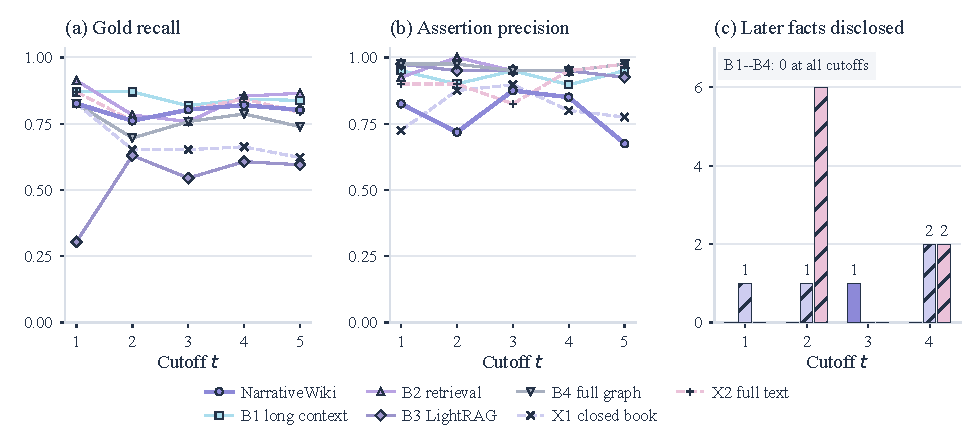
\includegraphics[width=\textwidth]{figures/f2-cutoff-anne.pdf}
\caption{Recall and precision at each cutoff (lines), and counts of assessed later facts
disclosed (bars). Dashed lines denote the X1 and X2 diagnostics. B1--B4 have zero observed
disclosures at every cutoff. Disclosure denominators are $|\Ft|=88,65,45,22$ at
$t=1,\ldots,4$; disclosure is undefined at $t=5$.}
\label{fig:cutoffplot}
\end{figure*}

Table~\ref{tab:full-results} reports the individual cells underlying the means in
Table~\ref{tab:main}; Figure~\ref{fig:cutoffplot} plots them. Long-context recall is
approximately stable across cutoffs. \sys has its highest recall on the first book, where it
matches the closed-book diagnostic, and its lowest at $t=2$. Closed-book recall declines from
the first book to the fifth. LightRAG's low recall at $t=1$ accompanies retrieved context
concentrated on the opening chapters. With only 40 sampled atoms per cell, the precision
results do not establish a trend across cutoffs. Every reported model call used the shared
generator. Table~\ref{tab:stats} gives the mean, standard deviation, median, minimum, and
maximum across cutoffs; Table~\ref{tab:paired} reports the same summaries for the paired
differences discussed in Section~\ref{sec:results}.
